\documentclass[xcolor=dvipsnames]{beamer}
\usepackage[titlepage=uibktitlepage1, titleRows=2, language=german]{uibkstyle}
\usepackage[utf8]{inputenc}
\usepackage{mathtools}

\newcommand{\semfootnote}[1]{\let\thefootnote\relax\footnotetext{#1}}

\makeatletter
\def\ScaleIfNeeded{%
\ifdim\Gin@nat@width>\linewidth
\linewidth
\else
\Gin@nat@width
\fi
}
\makeatother

\title{R-Paket für Kanalkodierung mit Blockkodes}
\author{Benedikt Wimmer}

\begin{document}

\begin{frame}[plain]
\maketitle
\end{frame}




\begin{frame}{Gliederung}
	\tableofcontents
\end{frame}

\section{Einführung in Kanalkodierung}

\begin{frame}
\includegraphics[width=\ScaleIfNeeded]{channel}
\end{frame}

\begin{frame}{Motivation und Ziel}
\begin{itemize}[<+->]
\item Kodierer sind hauptsächlich in der Hardware realisiert.
\item Schlecht nachzuvollziehen, Lehre bisher nur theoretisch.
\item \textbf{Ziel:} R-Paket zur Simulation und Visualisierung der Kanalkodierung.
\end{itemize}
\end{frame}

\begin{frame}{Grundlagen}
\begin{itemize}[<+->]
\item Kodierung als Abbildung $$ D^k \rightarrow K^n $$
\item Koderate R $$R = \frac{k}{n}$$
\item Hamming Distanz d für $x,y \in K$ $$d(x,y) \coloneqq \mid \{i \in \{1,...,n\} \mid x_i \neq y_i \} \mid  $$
\item Beispiel $$d(1011,1010) = 1$$
\end{itemize}
\end{frame}

\begin{frame}{Grundlagen - Fehlermodell}
\begin{itemize}[<+->]
\item Additive White Gaussian Noise (AWGN) $$ x_i = y_i + Z_i \sim \mathcal{N}(0,\sigma^2) $$
\item Signal-Rausch-Verhältnis $$SNR = 10\log_{10}\left(\frac{Signalleistung~S}{Rauschleistung~N}\right) dB$$
\item Shannon Grenze $$ C_{max} \leq B \log_2 \left(1 + \frac{S}{N}\right)$$
\end{itemize}
\end{frame}

\section{Blockkodes}

\begin{frame}{Blockkodes - Allgemeines}
\begin{enumerate}[<+->]
\item Nachricht in Blöcke aufteilen
\item Jeden Block kodieren / dekodieren
\item Blöcke zur kodierten / dekodierten Nachricht zusammensetzen
\end{enumerate}
\end{frame}

\begin{frame}{Blockkodes - Buchstabieralphabet}
\begin{center}
\begin{tabular}{l l}
\emph{Daten} & \emph{Kodierung} \\
\hline
\textbf{A} & \texttt{Anton} \\
\textbf{B} & \texttt{Berta} \\
\textbf{C} & \texttt{Cäsar} \\
. & .\\
. & .\\
. & .\\
\textbf{Z} & \texttt{Zeppelin} \\
\end{tabular}
\end{center}
\end{frame}

\subsection{Hamming-Kodes}

\begin{frame}{Hamming-Kodes}
\begin{itemize}[<+->]
\item Hamming-(n,k)-Kode mit $n = 2^m-1$ und $k = 2^m-m-1$
\item Hamming-Distanz $d=3$, kann 1 Fehler korrigieren.
\item Generatormatrix $G = \left(I_k \mid A\right)$
\item Kontrollmatrix $H = \left(A^T \mid I_m\right)$
\end{itemize}
\semfootnote{Quelle: [1]}
\end{frame}

\begin{frame}{Hamming-Kodes - (7,4)}

$$G = \begin{pmatrix}
1 & 0 & 0 & 0 & 0 & 1 & 1 \\
0 & 1 & 0 & 0 & 1 & 0 & 1 \\
0 & 0 & 1 & 0 & 1 & 1 & 0 \\
0 & 0 & 0 & 1 & 1 & 1 & 1 \\
\end{pmatrix}$$

\pause
$$H = \begin{pmatrix}
0 & 1 & 1 & 1 & \textcolor{red}{1} & 0 & 0 \\
1 & 0 & 1 & 1 & 0 & \textcolor{red}{1} & 0 \\
1 & 1 & 0 & 1 & 0 & 0 & \textcolor{red}{1}\\
\end{pmatrix}$$

\pause
$$H' = \begin{pmatrix}
0 & 0 & 0 & \textcolor{red}{1} & 1 & 1 & 1 \\
0 & \textcolor{red}{1} & 1 & 0 & 0 & 1 & 1 \\
\textcolor{red}{1} & 0 & 1 & 0 & 1 & 0 & 1 \\
\end{pmatrix}$$
\end{frame}

\begin{frame}{Hamming-Kodes - (7,4)}

$$G = \begin{pmatrix}
1 & 0 & 0 & 0 & \textcolor{green}{0} & \textcolor{green}{1} & \textcolor{green}{1} \\
0 & 1 & 0 & 0 & \textcolor{green}{1} & \textcolor{green}{0} & \textcolor{green}{1} \\
0 & 0 & 1 & 0 & \textcolor{green}{1} & \textcolor{green}{1} & \textcolor{green}{0} \\
0 & 0 & 0 & 1 & \textcolor{green}{1} & \textcolor{green}{1} & \textcolor{green}{1} \\
\end{pmatrix}$$

$$H = \begin{pmatrix}
\textcolor{green}{0} & \textcolor{green}{1} & \textcolor{green}{1} & \textcolor{green}{1} & \textcolor{red}{1} & 0 & 0 \\
\textcolor{green}{1} & \textcolor{green}{0} & \textcolor{green}{1} & \textcolor{green}{1} & 0 & \textcolor{red}{1} & 0 \\
\textcolor{green}{1} & \textcolor{green}{1} & \textcolor{green}{0} & \textcolor{green}{1} & 0 & 0 & \textcolor{red}{1}\\
\end{pmatrix}$$

\end{frame}

\begin{frame}{Hamming - (7,4) - Kodierung}
\[\begin{pmatrix}1\\0\\1\\0\\ \end{pmatrix}^T. \begin{pmatrix}1&0&0&0&\textcolor{red}{0}&\textcolor{green}{1}&\textcolor{blue}{1}\\0&1&0&0&\textcolor{red}{1}&\textcolor{green}{0}&\textcolor{blue}{1}\\0&0&1&0&\textcolor{red}{1}&\textcolor{green}{1}&\textcolor{blue}{0}\\0&0&0&1&\textcolor{red}{1}&\textcolor{green}{1}&\textcolor{blue}{1}\end{pmatrix} = \begin{pmatrix}1\\0\\1\\0\\\textcolor{red}{1}\\\textcolor{green}{0}\\\textcolor{blue}{1}\\ \end{pmatrix}^T\]
\end{frame}

\begin{frame}{Hamming - (7,4) - Dekodierung}
\[\begin{pmatrix}1\\0\\1\\0\\1\\0\\1\\ \end{pmatrix}^T. \begin{pmatrix}0&1&1&1&1&0&0\\1&0&1&1&0&1&0\\1&1&0&1&0&0&1\end{pmatrix} = \begin{pmatrix}\textcolor{green}{0}\\\textcolor{green}{0}\\\textcolor{green}{0}\\ \end{pmatrix}^T\]

Kodewort: (1,0,1,0,1,0,1)\\
Datenwort: (1,0,1,0)
\end{frame}

\begin{frame}{Hamming - (7,4) - Dekodierung}
\[\begin{pmatrix}1\\1\\1\\0\\1\\0\\1\\ \end{pmatrix}^T. \begin{pmatrix}0&\textcolor{red}{1}&1&1&1&0&0\\1&\textcolor{red}{0}&1&1&0&1&0\\1&\textcolor{red}{1}&0&1&0&0&1\end{pmatrix} = \begin{pmatrix}\textcolor{red}{1}\\\textcolor{red}{0}\\\textcolor{red}{1}\\ \end{pmatrix}^T\]

Kodewort: (1,1,1,0,1,0,1) \\ 
Fehlerindex: 2 \\ 
Korrigiertes Kodewort: (1,\textcolor{green}{0},1,0,1,0,1)\\
Datenwort: (1,\textcolor{green}{0},1,0)
\end{frame}

\subsection{BCH-Kodes}

\begin{frame}{BCH-Kodes}
\begin{itemize}[<+->]
\item \textbf{B}ose-\textbf{C}haudhuri-\textbf{H}ocquenghem
\item \textbf{(n,k,d)}-Kode
\item Korrigiert auf $n$-Bit Kodewörter bis zu $t=\frac{d}{2}-1$ Fehler
\end{itemize}
\end{frame}

\begin{frame}{BCH - Kodierung}
\begin{itemize}[<+->]
\item Nachrichten werden als Polynome mit Koeffizienten aus $GF(2)$ interpretiert.
\item Generatorpolynom $g(x)$ kodiert Datenwort $dw(x)$: $$kw(x) = dw(x)x^{n-k} - \left(dw(x)x^{n-k} \mod g(x)\right)$$
\end{itemize}
\end{frame}

\begin{frame}{BCH - (15,5,7) - Kodierung}
Input: (\textcolor{green}{1,0,1,0,1})

Daten Polynom: \[dw(x) = x^{4} + x^{2} + 1\]
\pause
Generator Polynom:
\[g(x) = x^{10} + x^{8} + x^{5} + x^{4} + x^{2} + x^{1} + 1\]
\[ dw^*(x) = dw(x)*x^{10} = x^{14} + x^{12} + x^{10}\] 
\pause
Rest Polynom:
\[r(x) = dw^*(x)\mod g(x) = x^{9} + x^{6} + x^{2} + x^{1} + 1\] 
\pause
Kode Polynom:
\[kw(x) = c( r(x)|dw(x) ) = x^{14} + x^{12} + x^{10} + x^{9} + x^{6} + x^{2} + x^{1} + 1\]
Output:
(\textcolor{red}{1,1,1,0,0,0,1,0,0,1,}\textcolor{green}{1,0,1,0,1})
\end{frame}

\begin{frame}{BCH - Generatorpolynom}
Körpererweiterung $GF(2^m)$ konstruieren. Beispiel für $m=3$:
\pause
\begin{center}
\begin{tabular}{c|c|c|c}
$\alpha^i$ & Polynom & Vektor & Minimalpolynom\\
\hline
- & 0 & 000 & - \\
$\alpha^0$ & $1$ & 100 & - \\
$\alpha^1$ & $x$ & 010 & $x^3+x+1$ \\
$\alpha^2$ & $x^2$ & 001  & $x^3+x+1$ \\
$\alpha^3$ & $x+1$ & 110  & $x^3+x^2+1$ \\
$\alpha^4$ & $x^2+x$ & 011  & $x^3+x+1$ \\
$\alpha^5$ & $x^2+x+1$ & 111  & $x^3+x^2+1$ \\
$\alpha^6$ & $x^2+1$ & 101  & $x^3+x^2+1$  \\
\end{tabular}
\end{center}
\end{frame}

\begin{frame}{BCH - Generatorpolynom}
\begin{itemize}[<+->]
\item Generatorpolynom für $t$-Fehler korrigierenden Kode hat Nullstellen $$\alpha^1,...,\alpha^{2t}$$
\item Für Minimalpolynome $\phi_i$: $$g(x) = LCM(\phi_1(x),\phi_2(x),...,\phi_{2t}(x))$$
\end{itemize}
\end{frame}

\begin{frame}{BCH - Dekodierung}
\begin{enumerate}[<+->]
\item Berechnen der Syndrome $S_i = kw(\alpha^i) \mid 1 \leq i \leq 2t$.
\item Bestimmen des Fehlerstellenpolynoms $\sigma(x)$. (Berlekamp-Massey-Algorithmus)
\item Ermitteln der Inversen der Nullstellen von $\sigma(x)$, diese entsprechen den Fehlerindizes $\alpha^i$. (Chien's Suche)
\item Korrigieren der Fehler im Kodewort an den Fehlerindizes.
\end{enumerate}
\semfootnote{Quelle: [2]}
\end{frame}

\begin{frame}{Verwendung von Blockkodes}

\begin{itemize}[<+->]
\item Hamming-Kodes fast nur zu Lehrzwecken.
\item Reed-Solomon-Kodes in der Datenspeicherung.
\item LDPC und Turbo-Kodes lösen Blockkodes ab.
\end{itemize}

\end{frame}

\section{R}

\begin{frame}{Programmiersprache R}
\begin{itemize}[<+->]
\item Ursprünglich für statistische Zwecke entwickelt.
\item Über 8000 Pakete auf den CRAN-Servern.
\item Bereits in Lehrveranstaltungen verwendet.
\end{itemize}
\semfootnote{Quelle: [3]}
\end{frame}

\begin{frame}{Entwicklungsumgebung RStudio}
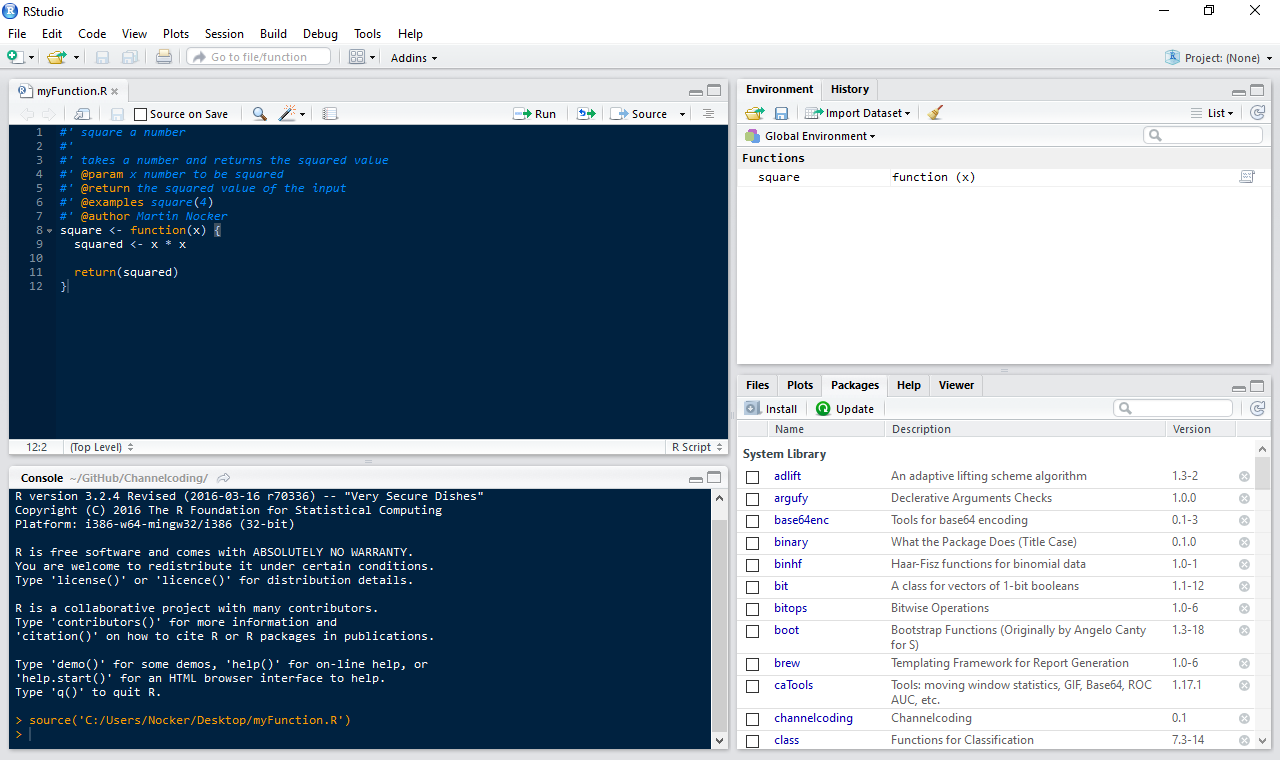
\includegraphics[width=\ScaleIfNeeded]{rstudio}
\end{frame}

\begin{frame}{Literatur}
\begin{itemize}
\item {[1]} Cary W. Huffman und Vera Pless. \emph{Fundamentals of error-correcting
codes.} Cambridge university press, 2010.
\item {[2]} Robert H. Morelos-Zaragoza. \emph{The art of error correcting coding.} John
Wiley and Sons, 2006.
\item {[3]} R Core Team. \emph{R: A Language and Environment for Statistical Computing.}
R Foundation for Statistical Computing. Vienna, Austria, 2016.
\end{itemize}
\end{frame}

\end{document}